\documentclass[12pt, handout]{beamer}
\useoutertheme{infolines} 
%\definecolor{grayish}{RGB}{147,162,153}
\usecolortheme[named=gray]{structure} 
\usetheme[height=7mm]{Rochester}

\usepackage{graphicx}

\usepackage{AMMALanguages}
\usepackage{hyperref}
\usepackage{tikz}
\usetikzlibrary{positioning}
\usetikzlibrary{arrows,shapes}

%\setbeameroption{show notes}
%\setbeameroption{show only notes}
\setbeamertemplate{note page}[plain]

\usepackage[utf8]{inputenc}
\usepackage[T1]{fontenc}

\usepackage{listings}
%\definecolor{commentcolor}{RGB}{78,156,93}

%used for ATL code listing
%\definecolor{darkgreen}{RGB}{14, 107, 57}
%\definecolor{keywordcolor}{RGB}{128, 0, 84}

\newcommand\blfootnote[1]{%
  \begingroup
  \renewcommand\thefootnote{}\footnote{#1}%
  \addtocounter{footnote}{-1}%
  \endgroup
}

\AtBeginSection{\frame{\sectionpage}}

\title[SyVOLT]{SyVOLT: Full Model Transformation Verification Using Contracts}
%\title{Full Verification of Model Transformation Contracts for Declarative ATL}
\author[Oakes, Lucio]{\textbf{Bentley James Oakes}, Levi L\'{u}cio}
%\subtitle{}
%\logo{}
\institute[]{McGill University, Montreal\\fortiss, Munich}
%\date{}
%\subject{}
%\setbeamercovered{transparent}
%\setbeamertemplate{navigation symbols}{}

% logo of my university
%\titlegraphic{\vspace{-0.5cm}
\includegraphics[width=3cm]{figures/mcgill}\hspace*{4.75cm}~%
%   
\includegraphics[width=4cm]{figures/big}
%}

% Abstract
%This talk will describe our method for statically verifying visual contracts on DSLTrans transformation. As DSLTrans is Turing-incomplete, this reduction in expressivity allows us to use a symbolic-execution approach to generate representations of all possible input models to the transformation. We then verify pre-/post-condition contracts on these representations, which in turn verifies the transformation itself.

%The technique we present is exhaustive for a DSLTrans transformation. This means that if the prover indicates a contract holds on a transformation, then the contract’s pre-/post-condition pair will be true for any input model for that transformation. We demonstrate our technique's applicability by displaying the results of verifying several relatively large model transformations, which have been translated from the ATL language. We also present our ‘slicing’ and 'pruning' optimization techniques, which restrict the number of symbolic executions the prover must consider. Finally, we finish by discussing our current efforts such as verifying contracts on the mbeddr DSL.



%show ATL code and DSLTRANS rule for country to community
%talk about dsltrans attributes

\begin{document}
\maketitle

%\section{Intro}

\begin{frame}{Motivation and Overview}
\begin{itemize}[<+->]
\item Model transformations are at the heart of model-driven engineering
\item Want to verify correctness for transformation specifications
\begin{itemize}[<+->]
\item Verify visual pre- / post-condition contracts
\item Identify those combinations of rules where contracts hold or not
\end{itemize}
\item Objective: Contract verification for all input models
\begin{itemize}
\item Input independence
\end{itemize}
\end{itemize}
\end{frame}


\section{DSLTrans and Symbolic Approach}




\begin{frame}{DSLTrans Transformation}

\begin{itemize}[<+->]
\item Visual language for model transformations

\item Graph-based, rule-based

\item Rules are grouped in sequential layers
\item Out-place so no rewriting performed
\begin{itemize}
\item Suited for `translation' transformations
\end{itemize}
\item All its computations are terminating and confluent
\begin{itemize}
\item Unbounded loops during execution are not allowed
\end{itemize}


\end{itemize}

\blfootnote{Selim, Gehan et al. "Model transformations for migrating legacy deployment models in the automotive industry." Software and Systems Modeling 14, no. 1 (2013): 365-381.}

\end{frame}


\begin{frame}{DSLTrans}
\begin{center}
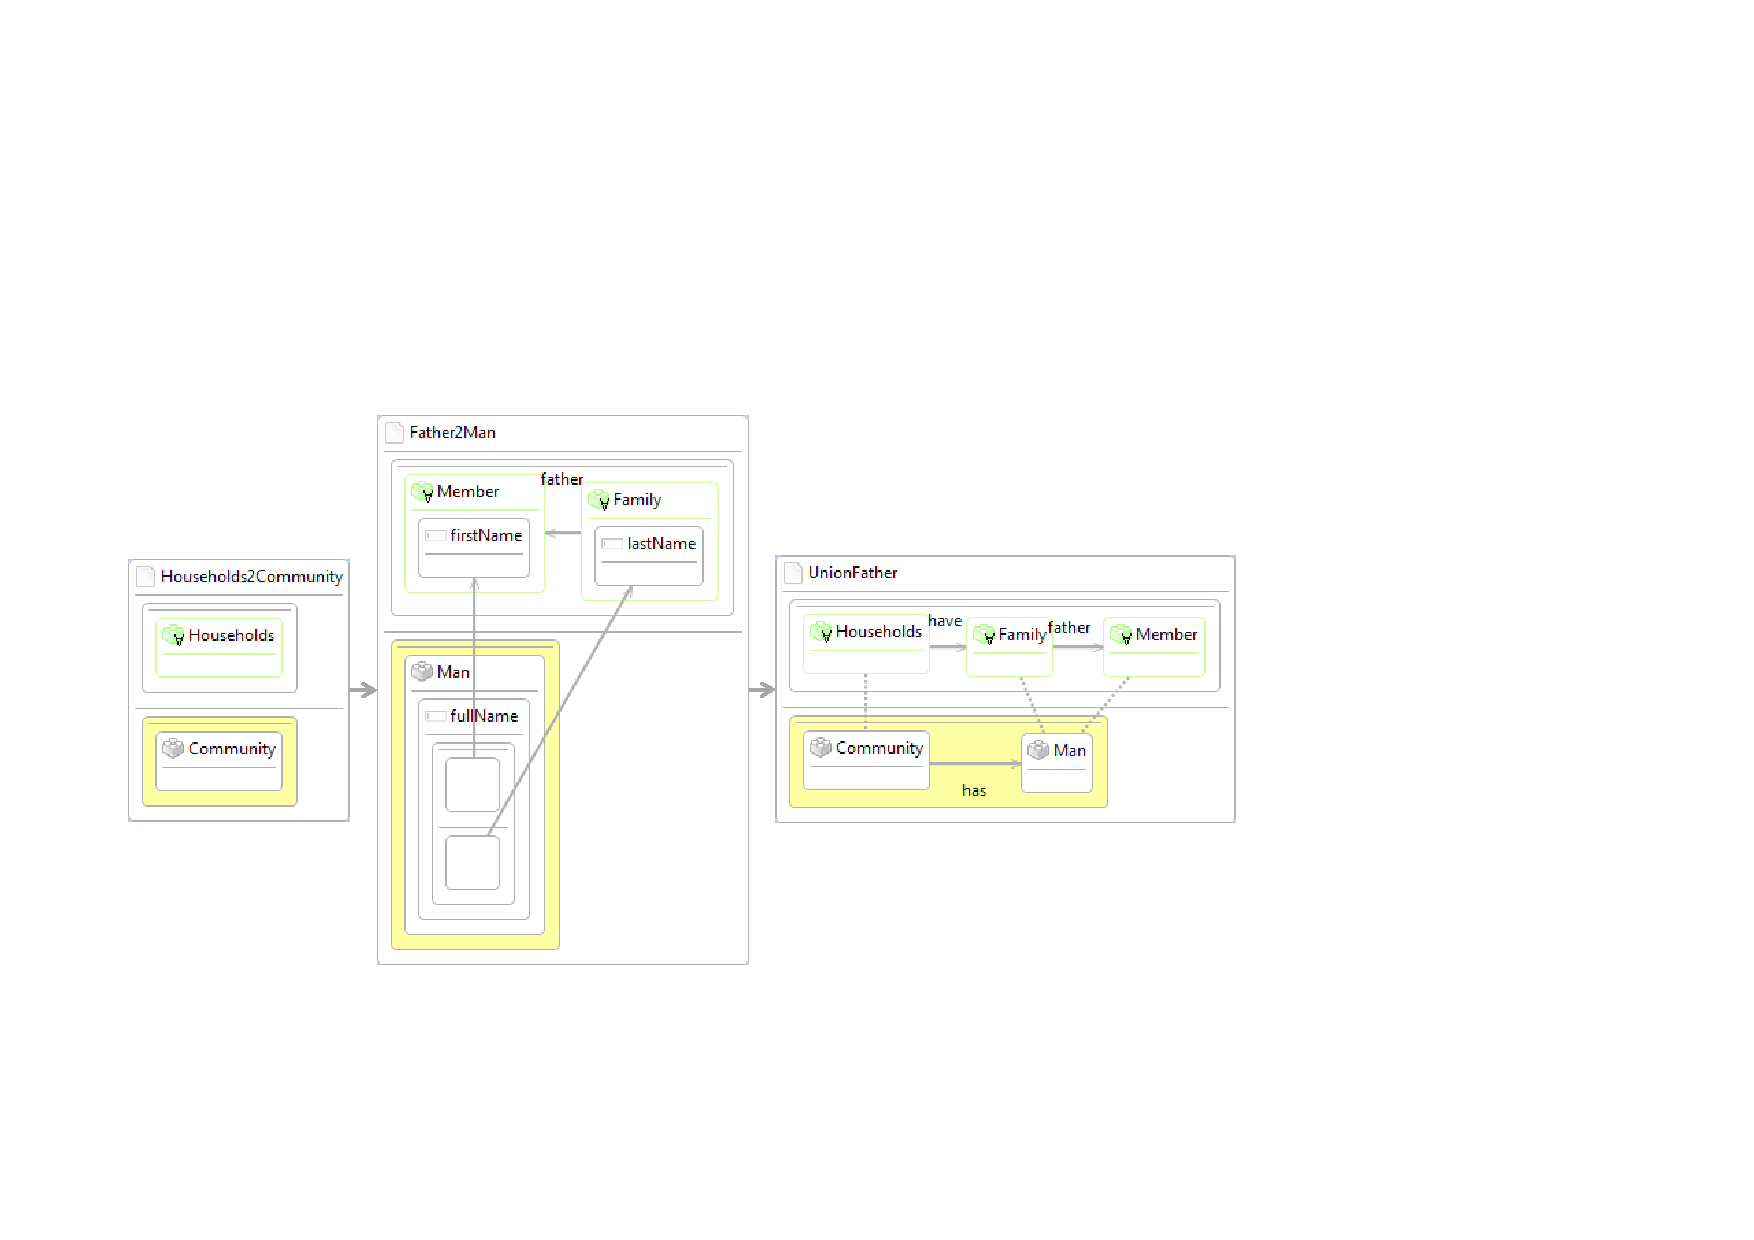
\includegraphics[width=\textwidth]{figures/Rules}
\end{center}
\pause
\begin{itemize}[<+->]
\item Rules arranged in layers
\item Match graph on top of rules
\item Apply graph on bottom
\begin{itemize}
\item Produced when match graph is found
\end{itemize}
\end{itemize}
\end{frame}

\section{Contracts}


\begin{frame}{Pre- / Post- Visual Contracts}
\begin{columns}[T] % contents are top vertically aligned
     \begin{column}[T]{0.45\textwidth} % each column can also be its own environment
     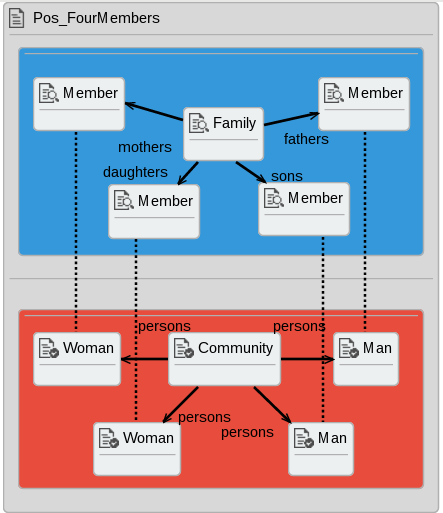
\includegraphics[width=\textwidth]{figures/Pos_FourMembers}
     \end{column}
     \begin{column}[T]{0.55\textwidth}
     \begin{itemize}[<+->]
     \item If blue graph is found in input model, then red graph is found in output model
     \item Objective: Prove for all input models/transformation executions - input independence
     \item \textit{A family with a father, mother, son, daughter
     should always produce two males and two females in the
     target community}
     \end{itemize}
     \end{column}
     \end{columns}

\end{frame}

\begin{frame}{Pattern Contracts}
\begin{center}
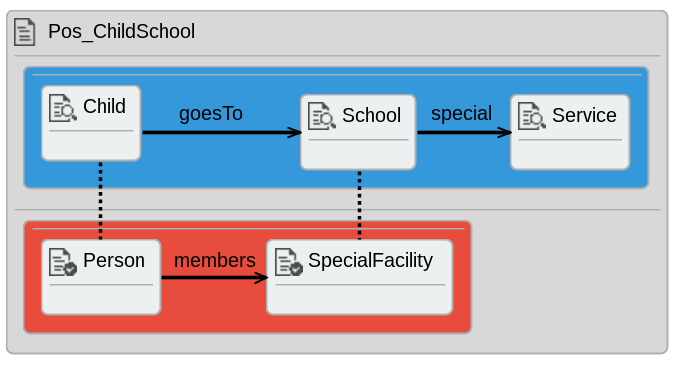
\includegraphics[width=0.65\textwidth]{figures/Pos_ChildSchool}
\end{center}
\begin{itemize}
\item Relates elements in input model to elements in output model
\item \textit{If a Child goesTo a School that has a special Service, then a SpecialFacility has the associated Person as a member}
\item Intention is to allow verification of rule interaction
\begin{itemize}
\item Three rules in example
\end{itemize}
\end{itemize}
\end{frame}


\begin{frame}{Element Attributes}
\begin{center}
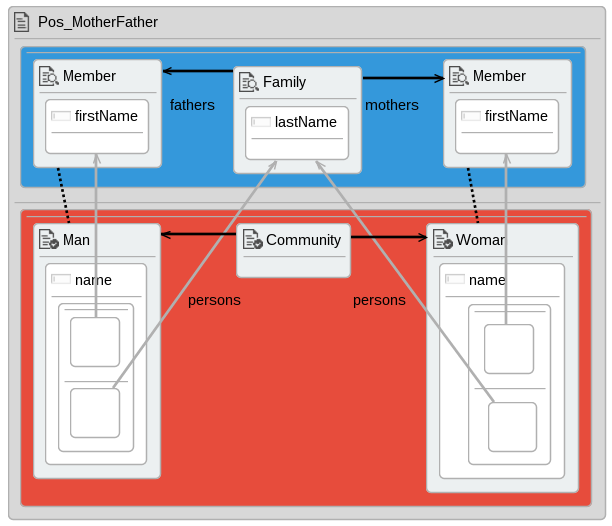
\includegraphics[width=0.50\textwidth]{figures/Pos_MotherFather}
\end{center}
\pause
\begin{itemize}[<+->]
\item Reasoning about (String) attributes of elements
\item \textit{Is the full name of the produced Person correctly created from the last name of the Family and the first name of the Member?}
\end{itemize}
\end{frame}

\begin{frame}{Propositional Logic and Pivots}
\begin{center}
\begin{center}
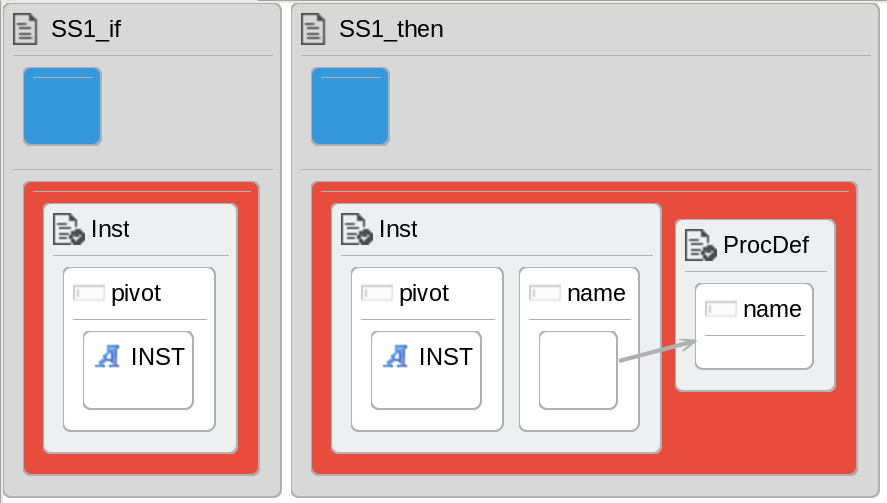
\includegraphics[width=0.7\textwidth]{figures/syntactic_invariant}
\end{center}
\end{center}
\pause
\begin{itemize}[<+->]
\item Contracts can be combined with AND, OR, NOT, IF-THEN
\item Pivots ensure that same element is bound in both contracts
\item  \textit{If there is an Inst element, then that Inst element has the same name as a ProcDef element}
\end{itemize}
\end{frame}

\begin{frame}{Syntactic Invariants}
\begin{center}
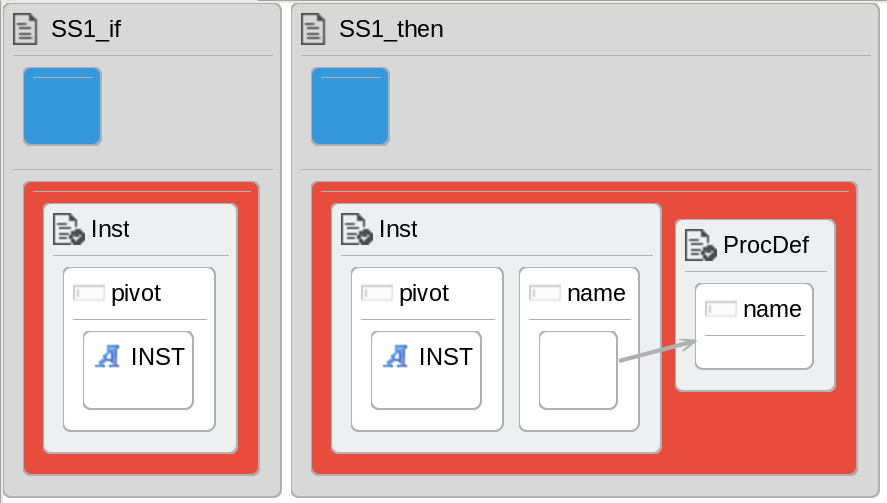
\includegraphics[width=0.7\textwidth]{figures/syntactic_invariant}
\end{center}
\begin{itemize}
\item Check if path condition has well-formed input or output syntax
\item \textit{If there is an Inst element, then that Inst element has the same name as a ProcDef element}
\end{itemize}
\end{frame}

%\begin{frame}{Multiplicity Invariants}
%\begin{center}
%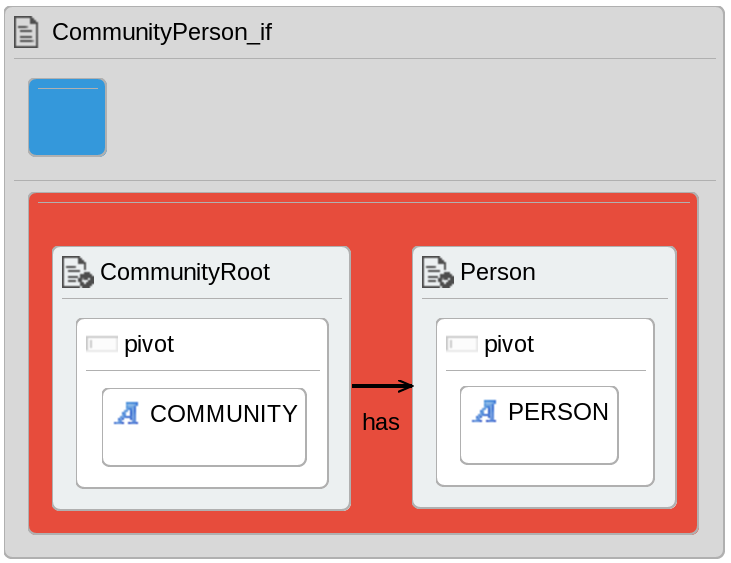
\includegraphics[width=0.45\textwidth]{figures/communityPersonProp_if}
%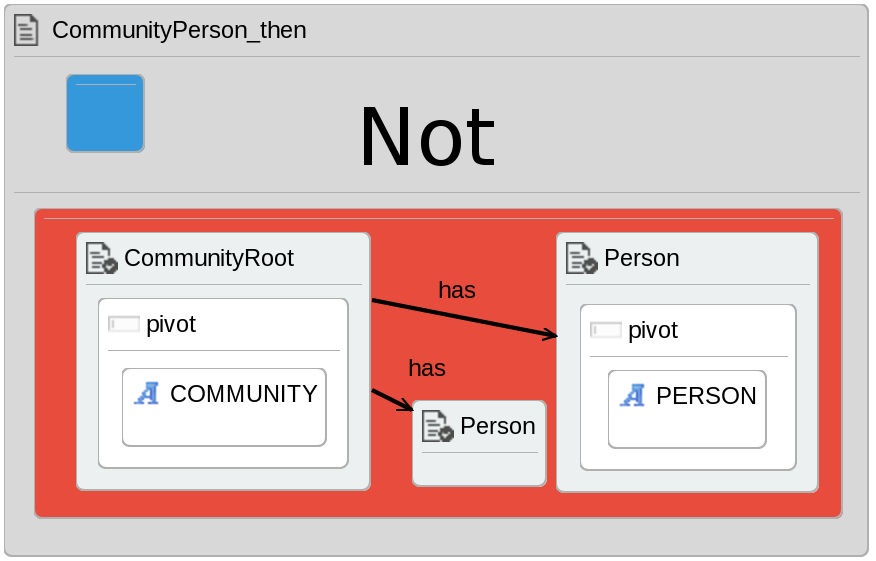
\includegraphics[width=0.45\textwidth]{figures/communityPersonProp_then}
%\end{center}
%\begin{itemize}
%\item \textit{Only one Person is in the Community in the output model}
%\end{itemize}
%\begin{itemize}
%\item Abstraction of our approach loses multiplicity information
%\begin{itemize}
%\item Multiple applications of a rule are not represented
%\end{itemize}
%\item Contract only fails if \textit{two Persons are always created in output}
%\end{itemize}
%\end{frame}

\section{SyVOLT}

\begin{frame}{SyVOLT Tool}
\begin{itemize}[<+->]
\item All possible executions of the transformation are symbolically constructed
\begin{itemize}[<+->]
\item Built as sets of rules called path conditions
\begin{itemize}
\item No rules execute, only rule 1 executes, rule 1 and rule 2 both execute
\end{itemize}
\item Rule dependencies/combinations resolved

\end{itemize}
\item Final finite set of path conditions represents all possible transformation executions

\end{itemize}

\begin{center}
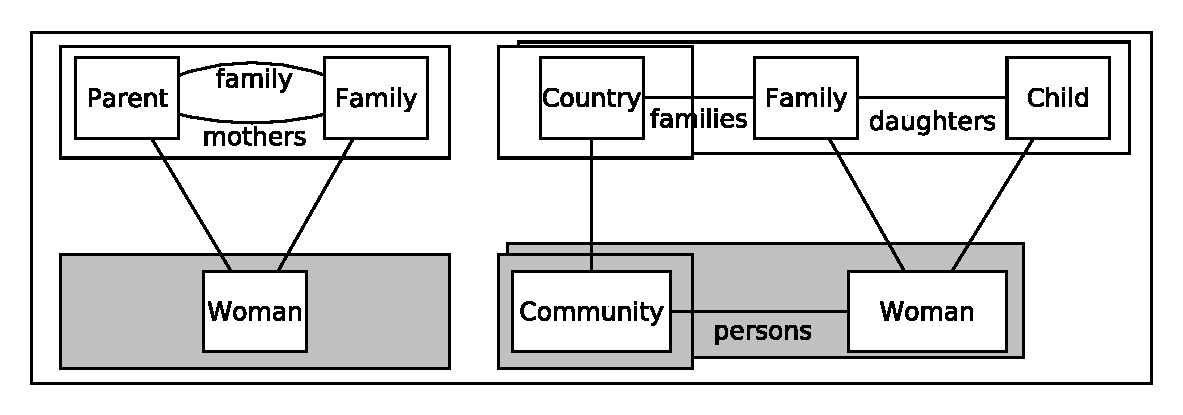
\includegraphics[width=0.8\textwidth]{figures/pc}
\end{center}

\begin{itemize}
\item Path condition representing execution of three rules
\end{itemize}
\end{frame}

\begin{frame}{SyVOLT Tool}
\begin{itemize}[<+->]
\item A contract holds for a transformation if it holds for all generated path conditions
\begin{itemize}
\item Contract is matched onto path condition
\end{itemize}
\item Otherwise, counter-example path conditions are produced
\item Proving process completes within seconds
\end{itemize}
\blfootnote{L. Lúcio, B. Oakes, and H. Vangheluwe. A technique for symbolically verifying properties of graph-based model transformations. Technical report, Technical Report SOCS-TR-2014.1, McGill U, 2014.}
\end{frame}

\begin{frame}{Contract Proving Example}
\begin{center}
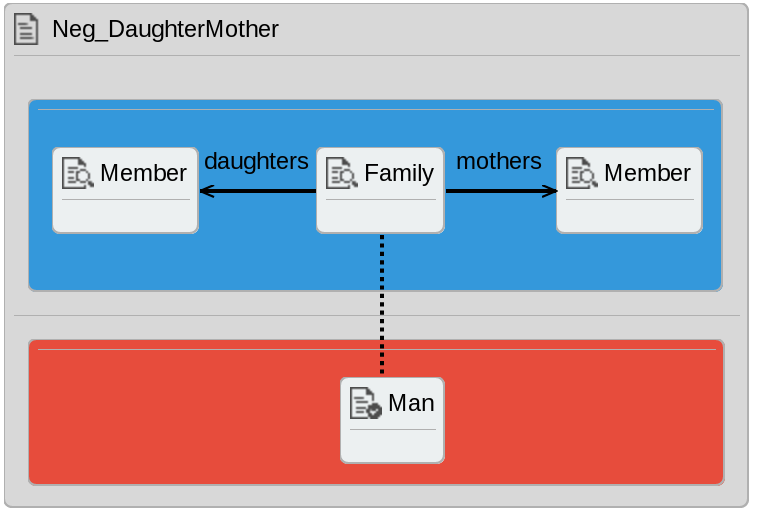
\includegraphics[width=0.7\textwidth]{figures/Pos_DaughterMother}
\end{center}
\begin{itemize}[<+->]
\item Statement: \textit{A family with a mother and a daughter will always produce a community with a man}
\item Fails on path condition: `HFamComm\_HMotherRule\_HDaughterRule'
\end{itemize}
\end{frame}

\section{ATL Experiments}

\begin{frame}{ATL}

\begin{itemize}[<+->]
\item Translating declarative ATL transformation into DSLTrans language
\item Verify visual contracts on DSLTrans
\end{itemize}
\begin{center}
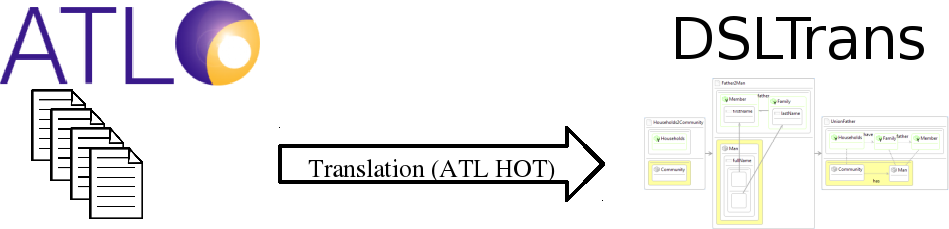
\includegraphics[width=\textwidth]{figures/overview}
\end{center}
\begin{itemize}[<+->]
\item Performed through a higher-order transformation
\begin{itemize}
\item Specified in ATL
\item DSLTrans transformations produced are equivalent to hand-built versions
\end{itemize}
\end{itemize}
\end{frame}


\begin{frame}{Rules Example}
\begin{columns}[T] % contents are top vertically aligned
     \begin{column}[T]{0.5\textwidth} % each column can also be its own environment
     \begin{center}
     
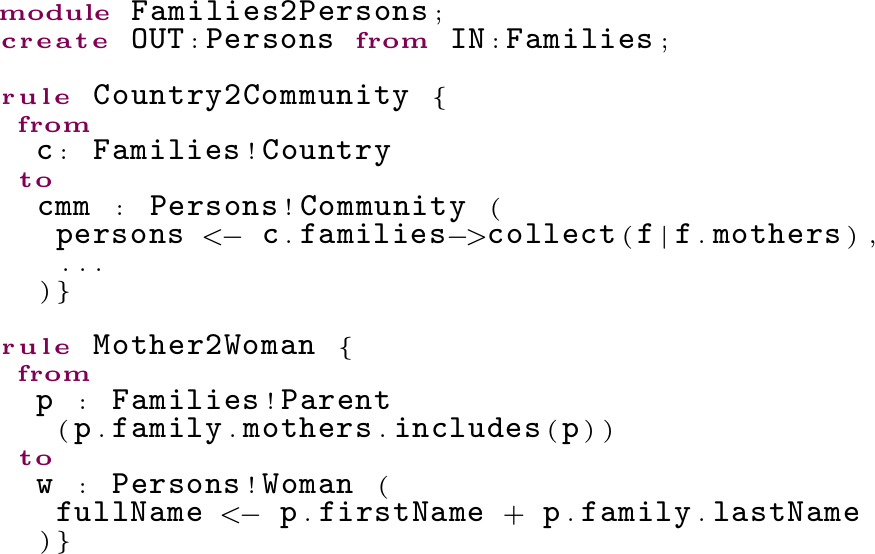
\includegraphics[width=0.98\textwidth]{figures/ATL_example}

     \end{center}
 \end{column}
     \begin{column}[T]{0.5\textwidth}
    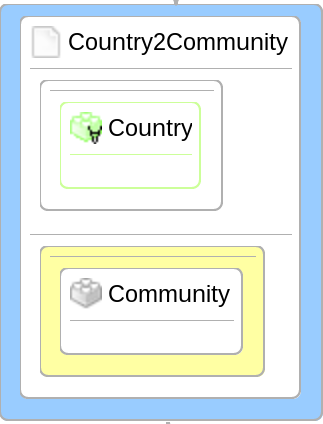
\includegraphics[height=0.45\textheight]{figures/Country2Community} \newline
     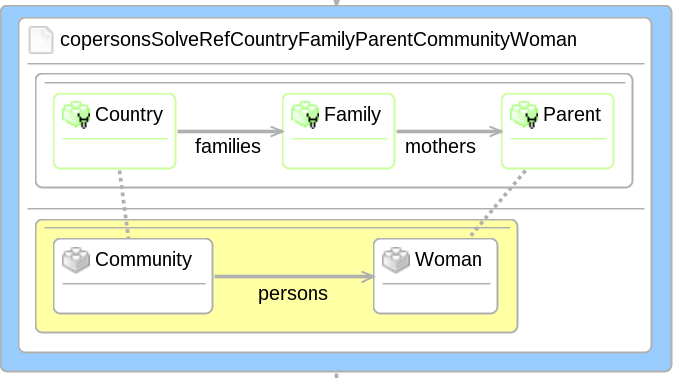
\includegraphics[height=0.45\textheight]{figures/copersonsWoman}
 \end{column}
 \end{columns}
\end{frame}




\begin{frame}{Performance}
\begin{center}
\tiny
\begin{tabular}{l | c| | r |r || r |r || r}
 &  \textbf{ATL/ DSLTrans}&  \textbf{Path Conds.}  & \textbf{Time (s)} & \textbf{Contracts} & \textbf{Time (s)}& \textbf{Memory}\\
 & \centering \textbf{Rules}&  \textbf{Generated}&  &  \textbf{Proved}& & \textbf{(MB)} \\ \hline\hline
Families2Person & \centering 5 / 9 & 101 & \textbf{0.24} & 4 & \textbf{0.52}& 54\\\hline
Ex. Families2Person & \centering10  / 19 & 366	& \textbf{3.89} & 10	&\textbf{ 7.35} & 59\\\hline
GM2AUTOSAR (handbuilt)& \centering5 / 9 & 13 & \textbf{0.18} & 9 &\textbf{ 0.15} & 58\\
GM2AUTOSAR (HOT)& \centering5 / 9 & 10 & \textbf{0.26} & 9 & \textbf{0.15} & 60\\\hline
UM2Kiltera & \centering20 / 17 & 322 & \textbf{1.86} & 15 & \textbf{11.99 }& 55\\
\end{tabular}
\end{center}

\begin{itemize}
\item Verified ATL contracts ranging from 5 to 20 rules
\item Time and memory requirements are feasible
\begin{itemize}
\item Experiments performed on 2013 Macbook Air
\end{itemize}
\end{itemize}
\end{frame}

\section{Verification Optimizations}

\begin{frame}{Slicing Transformation}
\begin{columns}[T] % contents are top vertically aligned
     \begin{column}[T]{0.45\textwidth} % each column can also be its own environment
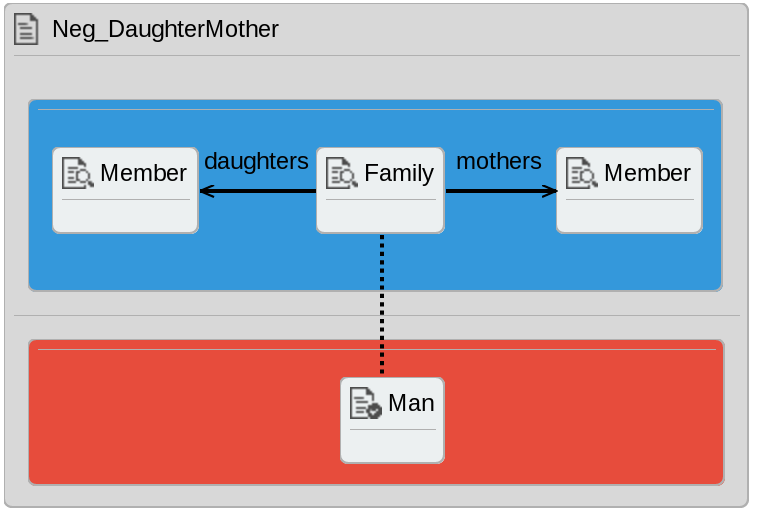
\includegraphics[width=0.9\textwidth]{figures/Pos_DaughterMother} \newline
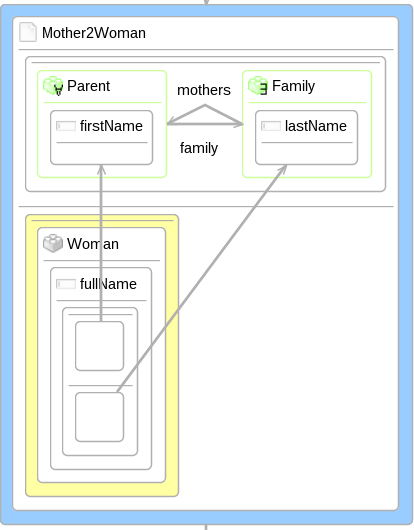
\includegraphics[width=0.9\textwidth]{figures/Mother2Woman}
 \end{column}
     \begin{column}[T]{0.55\textwidth}
     \begin{itemize}[<+->]
\item Core idea:
\begin{itemize}[<+->]
\item Symbolically execute only those rules which are necessary for the contract to be proven

\end{itemize}
\item Example:
\begin{itemize}
\item The contract contains a \textit{mothers} association
\item The rule matches over a \textit{mothers} association
\item Thus, we should consider this rule in our symbolic execution
\end{itemize}
\item Does this rule depend on any other rules?
\end{itemize}
 \end{column}
 \end{columns}
\end{frame}

\begin{frame}{Slicing Transformation}
\begin{columns}[T] % contents are top vertically aligned
     \begin{column}[T]{0.45\textwidth} % each column can also be its own environment
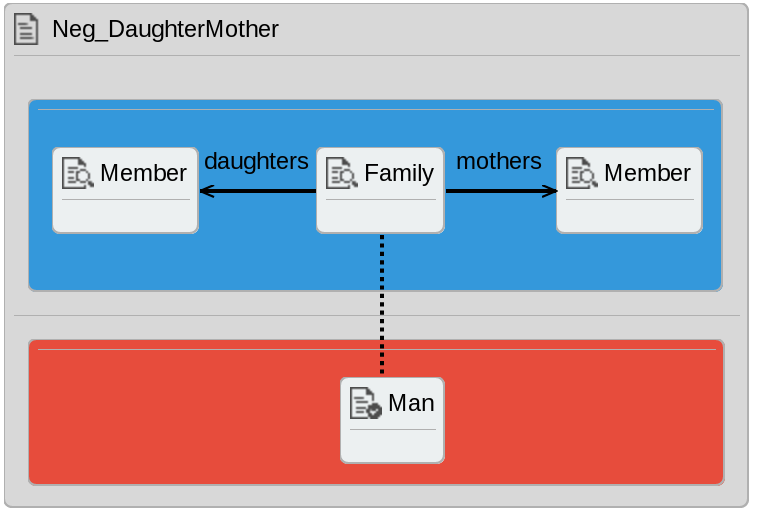
\includegraphics[width=0.9\textwidth]{figures/Pos_DaughterMother} \newline
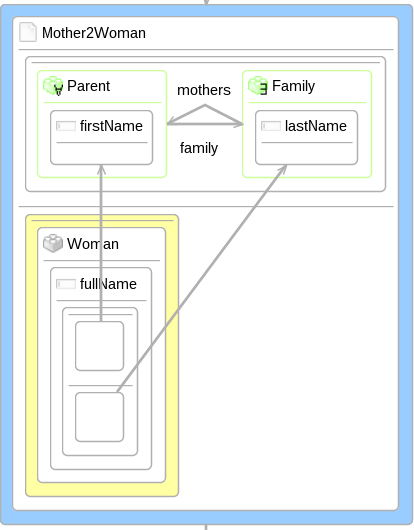
\includegraphics[width=0.9\textwidth]{figures/Mother2Woman}
 \end{column}
     \begin{column}[T]{0.55\textwidth}
     \begin{itemize}[<+->]
\item Procedure:
\begin{itemize}[<+->]
\item Decompose contracts and rules into elements
\item Record which rules produce these elements
\item Build a dependency graph
\item The rules in the graph must be symbolically executed
\end{itemize}
\item Automated process
\item Must be conservative
\end{itemize}
 \end{column}
 \end{columns}
\end{frame}

\begin{frame}{Slicing Results}

\begin{center}

\begin{tabular}{l l | r| r | r | r }
\textbf{Name} & \textbf{Version} & \textbf{Rules} & \textbf{PCs} & \textbf{PC Build}   & \textbf{Prove}\\
& & & &\textbf{Time (s)}&\textbf{Time (s)}\\\hline\hline
Contract 1& \textit{Original} & 17 & 322 & 1.47 & 5.29 \\
& \textit{Sliced}& 2 & 3 & 0.05 & 0.09 \\\hline

Contract 2& \textit{Original} & 17 & 322 & 1.68 & 7.01 \\
& \textit{Sliced}& 8 & 64 & 0.13 & 0.12 \\\hline

Contract 3 & \textit{Original} & 17 & 322 & 1.87 & 7.06\\
& \textit{Sliced}& 11 & 64 & 0.55 & 0.62 \\\hline
\end{tabular}
\end{center}

\begin{itemize}
\item Substantial reduction in path conditions created
\item Corresponding reduction in proving time
\end{itemize}
\end{frame}



\begin{frame}{Pruning}

\begin{itemize}
\item Core idea: Use metamodels to discard invalid output models
\item Example: a \textit{Man} is contained by a \textit{Community} through the \textit{persons} association
\item Any output model that has a \textit{Man} without \textit{persons} is invalid
\end{itemize}
\begin{center}
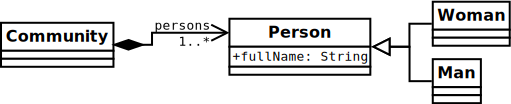
\includegraphics[width=\textwidth]{figures/PersonsMM}
\end{center}


\end{frame}

\begin{frame}{Pruning}
\begin{itemize}

\item Find containment links between classes in metamodel
\item Examine path conditions for missing containment links
\item Are there still rules that can be symbolically executed to build links?
\item If not, the output model is not valid, and that branch can be pruned

\end{itemize}
\begin{center}
%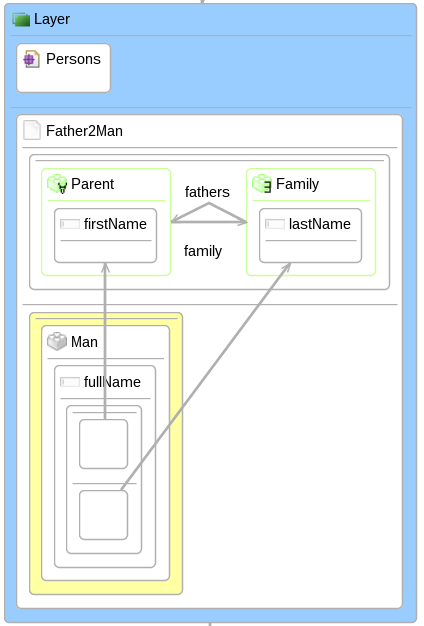
\includegraphics[width=0.35\textwidth]{figures/Father2Man}
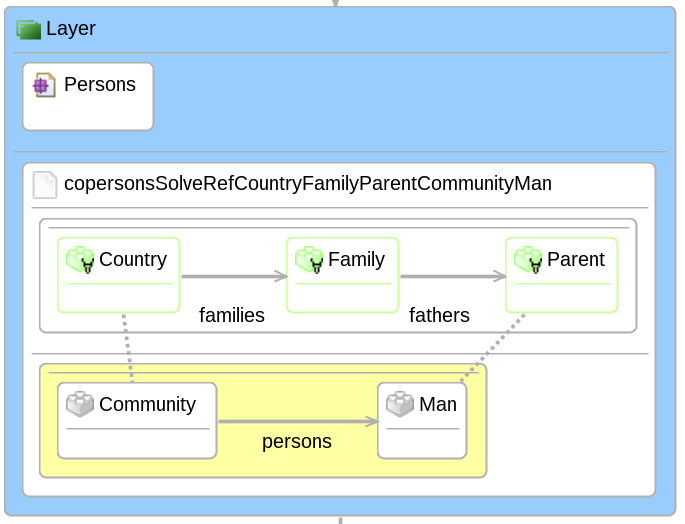
\includegraphics[width=0.5\textwidth]{figures/copersonsMan}
\end{center}

%\begin{itemize}
%\item Whenever left rule symbolically executes, right rule must also symbolically execute
%\end{itemize}
\end{frame}

\section{Current Work}




\begin{frame}{Eclipse Plugin}
\begin{center}
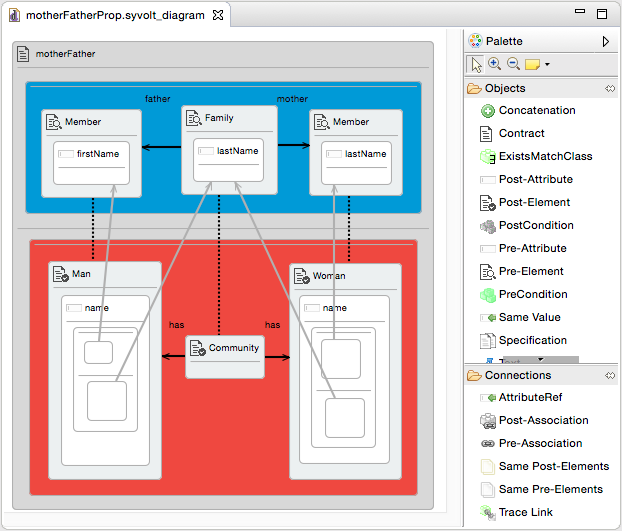
\includegraphics[height=0.8\textheight]{figures/eclipse_frontend}
\end{center}

\begin{itemize}
\item Eclipse GMF plugin for building DSLTrans transformations and contracts.
\end{itemize}
\end{frame}

\begin{frame}{MPS Plugin}
\begin{center}
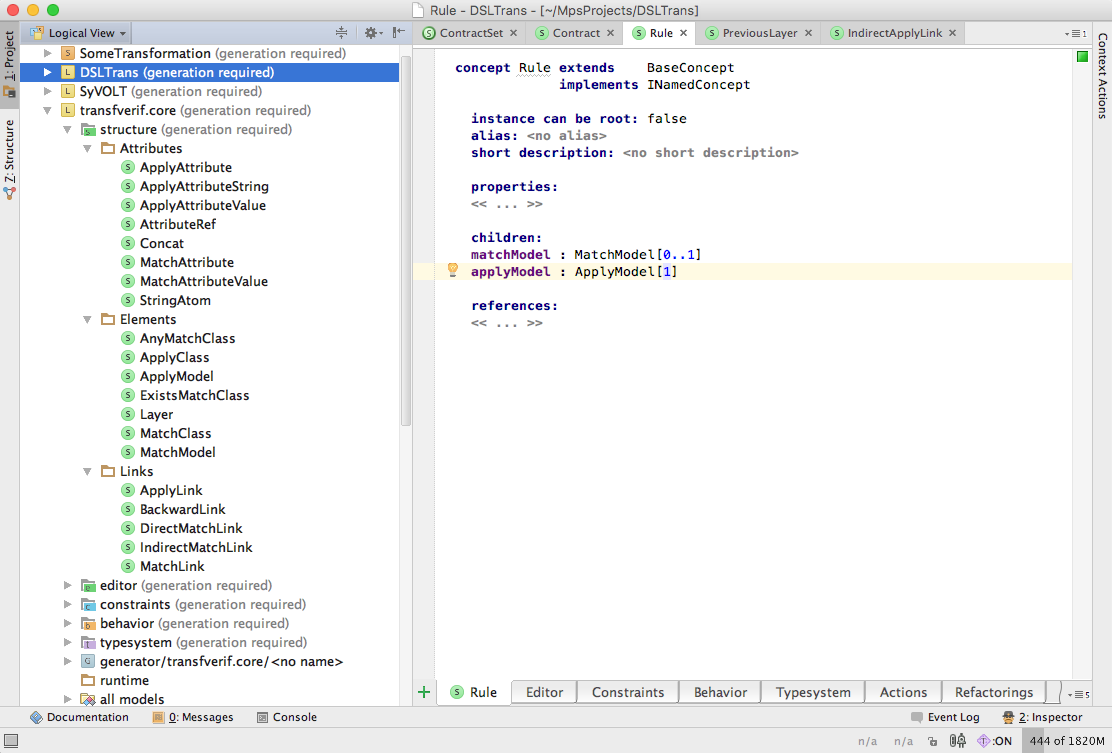
\includegraphics[height=0.8\textheight]{figures/DSLTransMPS}
\end{center}

\begin{itemize}
\item Levi Lucio is implementing DSLTrans as the model-to-model generator in MPS
\end{itemize}
\end{frame}

\begin{frame}{mbeddr DSLTrans Transformation}
\begin{center}
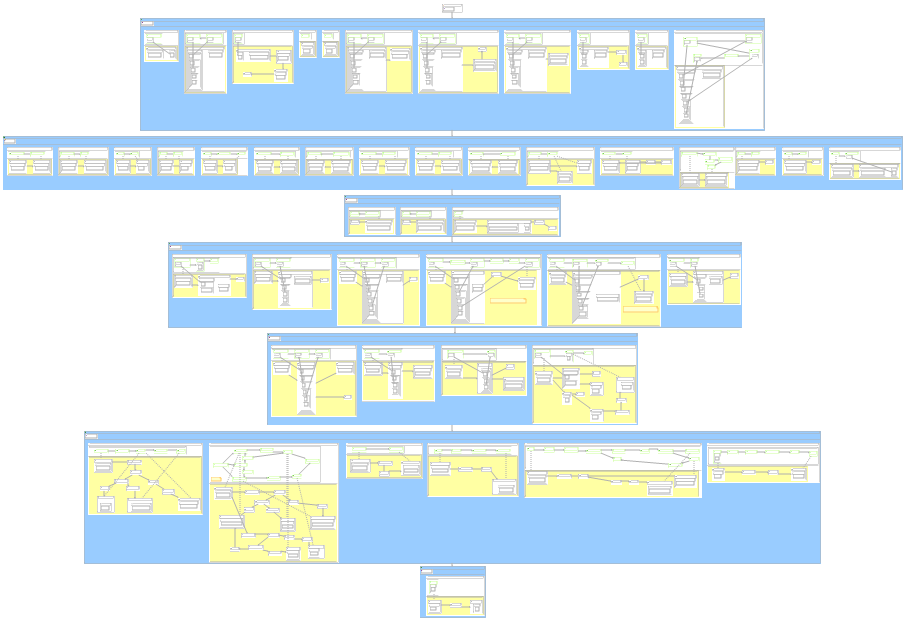
\includegraphics[width=0.8\textwidth]{figures/mbeddr}
\end{center}

\begin{itemize}
\item Verifying the C generator for the mbeddr DSL stack implemented in MPS
\end{itemize}
\end{frame}

\begin{frame}{Literature}
\small
\begin{itemize}[<+->]

\item Fuly Verifying Transformation Contracts for Declarative ATL\\
Bentley James Oakes, Javier Troya, Levi Lucio, and Manuel Wimmer\\
Proceedings of MODELS 2015
\begin{itemize}
\item Extended to journal article: Full Contract Verification for ATL using Symbolic Execution, SoSyM (to appear)
\end{itemize}
\item  Finding and Fixing Bugs in Model Transformations with Formal Verification: An Experience Report\\
Gehan M. K. Selim, James R. Cordy, Juergen Dingel, Levi Lucio and Bentley James Oakes\\
Proceedings of AMT 2015
\end{itemize}
\end{frame}


\begin{frame}{Conclusion}
\begin{itemize}[<+->]
\item Verification of visual contracts on DSLTrans transformations
\item Approach is complete for all transformation executions
\item Can extend contract language expressiveness
\item Eclipse plugin to build transformation and contracts
\item Current work: Verification of mbeddr transformation
\end{itemize}
\pause
\begin{itemize}
\item Thank you for your time!
\end{itemize}
\begin{center}
\textbf{SyVOLT: Full Model Transformation Verification Using Contracts}\\
\end{center}
\end{frame}


%\begin{frame}{Contract Expressibility}
%
%\begin{itemize}[<+->]
%\item Next few slides will discuss concepts expressible with our contract language.
%
%\begin{itemize}[<+->]
%\item Pattern contracts
%\item Element attributes
%\item Propositional logic and pivots
%\item Syntactic invariants
%\item Multiplicity invariants
%\end{itemize}
%\end{itemize}
%
%\begin{itemize}
%\item Prover reports rule reachability as well
%\end{itemize}
%
%\blfootnote{Selim, G.M.: Formal Verification of Graph-Based Model Transformations. Ph.D. thesis, Queen’s University. 2015.}
%\end{frame}


\begin{frame}{Multiplicity Invariants}
\begin{center}
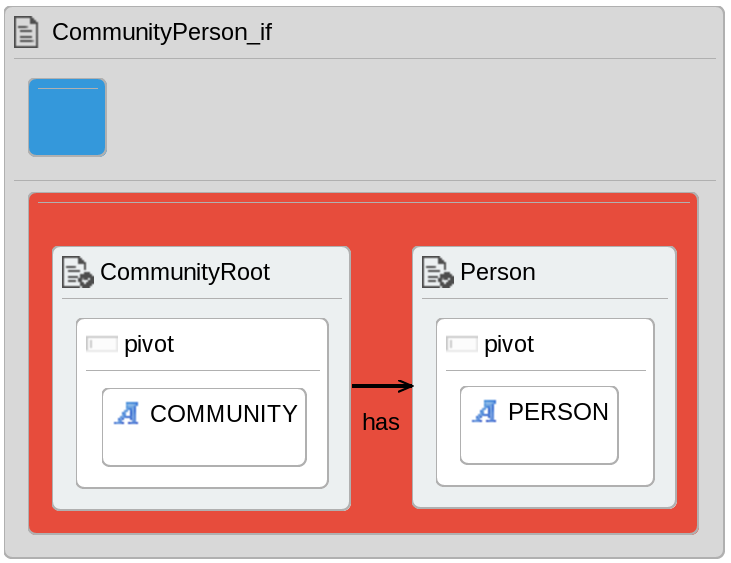
\includegraphics[width=0.45\textwidth]{figures/communityPersonProp_if}
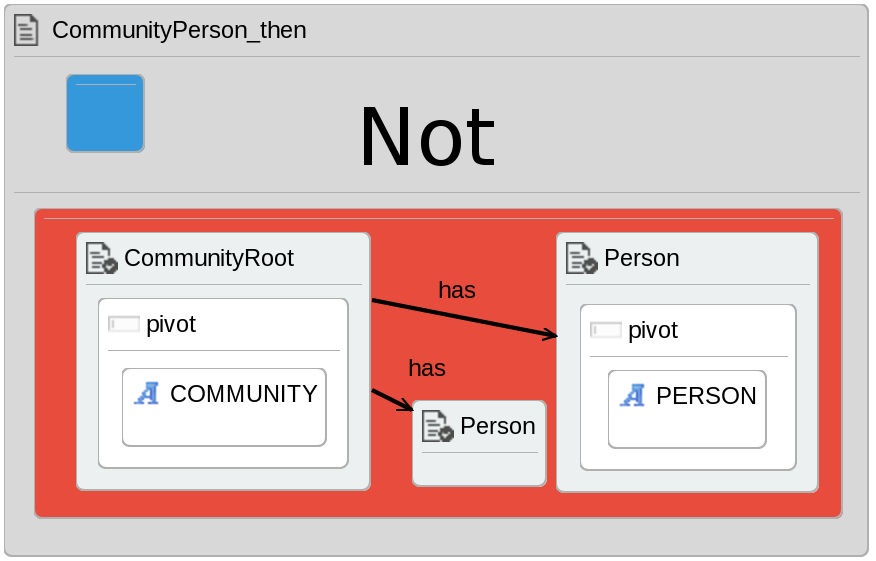
\includegraphics[width=0.45\textwidth]{figures/communityPersonProp_then}
\end{center}
\begin{itemize}
\item \textit{Only one Person is in the Community in the output model}
\end{itemize}
\begin{itemize}
\item Abstraction of our approach loses multiplicity information
\begin{itemize}
\item Multiple applications of a rule are not represented
\end{itemize}
\item Contract only fails if \textit{two Persons are always created in output}
\end{itemize}
\end{frame}


\begin{frame}{Contract Limitations}

\begin{itemize}
\item DSLTrans transformation language only manipulates Strings
\begin{itemize}
\item Could pack data and operations into Strings
\end{itemize}
\end{itemize}

\begin{itemize}
\item Limitations from symbolic execution technique
\begin{itemize}
\item Loses multiplicity information
\begin{itemize}
\item Cannot count elements created
\item Difficult to express \textit{for each A element, there exists unique B element}
\end{itemize}
\end{itemize}
\end{itemize}

\end{frame}

\begin{frame}{Contract Limitations}

\begin{itemize}
\item No query language implemented
\begin{itemize}
\item Cannot create sets of elements
\item Cannot match pattern with inheritance and report subtype names
\item No indirect links/navigation
\end{itemize}
\item Difficult to reason about negative contracts
\item Cannot validate instance data
\begin{itemize}
\item `Do all names start with G'
\item `Is gender == male or age < 18'
\end{itemize}
\end{itemize}

\end{frame}

\end{document}
